%!LW recipe=pdflatex ➞ bibtex ➞ pdflatex`×2

\documentclass[twocolumn]{article}

\usepackage[backend=bibtex]{biblatex} 
\usepackage{kpfonts} 
\usepackage{amsmath}
\usepackage[margin=2cm]{geometry} 
\usepackage{hyperref} 
\usepackage{siunitx} 
\usepackage{graphicx} 
\usepackage[super]{nth} 
\usepackage{tabularx} 
\usepackage{ltablex} 
\usepackage{longtable} 
\usepackage{subcaption} 
\usepackage{booktabs}
\usepackage{multirow}
\usepackage{svg}
\usepackage{float}

\addbibresource{refs.bib}

\title{Convolutional LSTM For Image Sequence Modelling}
\author{Henry Williams}
\date{\today}

\begin{document}
\maketitle

\section{Introduction}

In this report, we outline and evaluate our implementation of a Convolutional Long-Term-Short-Term Memory (LSTM) model for image sequence modelling. We develop a model which learns both \emph{extrapolation} and \emph{interpolation} of images within a dataset based on MNIST with autoregressive transformations applied at each time step. We also perform a rigorous evaluation of our model, with both quantitative and qualitative analysis, and analyse its robustness to both noise and missing data\footnote{The code for our models, training, generation of graphs, and results can be found at the following GitHub repository: \url{https://github.com/Henry-Ash-Williams/amml-assessment}}. 

\section{Background}

Sequence modelling consider data which change over a given time. For example, this could include predicting the movement of a stocks price given its historical movements~\cite{nelson2017stock}, or captions given some audio~\cite{drossos2017automated}. 

One of the earliest approaches for sequence modelling using neural networks, known as Recurrent Neural Networks (RNNs), take the hidden representation of the previous element in the sequence, $h_{t-1}$, in addition to the current element $x_t$ to produce the output of the sequence, $y_t$ (Figure~\ref{fig:rnn}). Using a variation of the backpropagation algorithm, known as backprop-through-time, RNNs can learn to effectively model a sequence of data~\cite{mozer1995bptt}.

\begin{figure}[h]
    \centering
    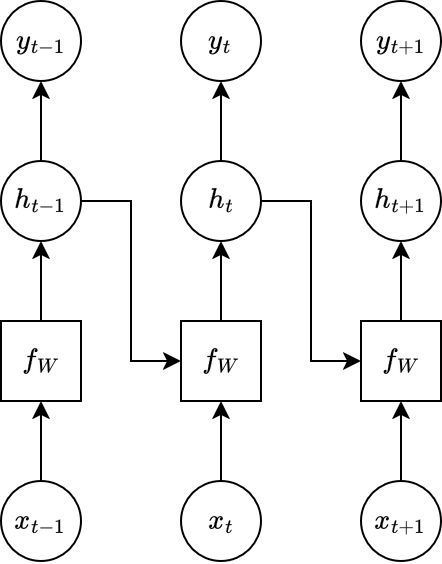
\includegraphics[scale=0.25]{assets/rnn.png}
    \caption{Model Diagram of a Reccurent Neural Network}
    \label{fig:rnn}
\end{figure}

However, these models often suffer from the problems of both exploding and vanishing gradients. The exploding gradient problem can be mitigated using gradient clipping, the latter however, poses a more pertinant challenge. One solution to this problem, known as an LSTM~\cite{hochreiter1997long}, replaces the recurrent connection with a memory cell, and enable the model to learn what should be remembered, and what should forgotten. The hidden and cell states, $h_t$ and $c_t$ respectively, given the current input, $x_t$, and previous hidden and cell states, are shown in Equation~\ref{eq:lstm}. 

\begin{figure}
    \centering
    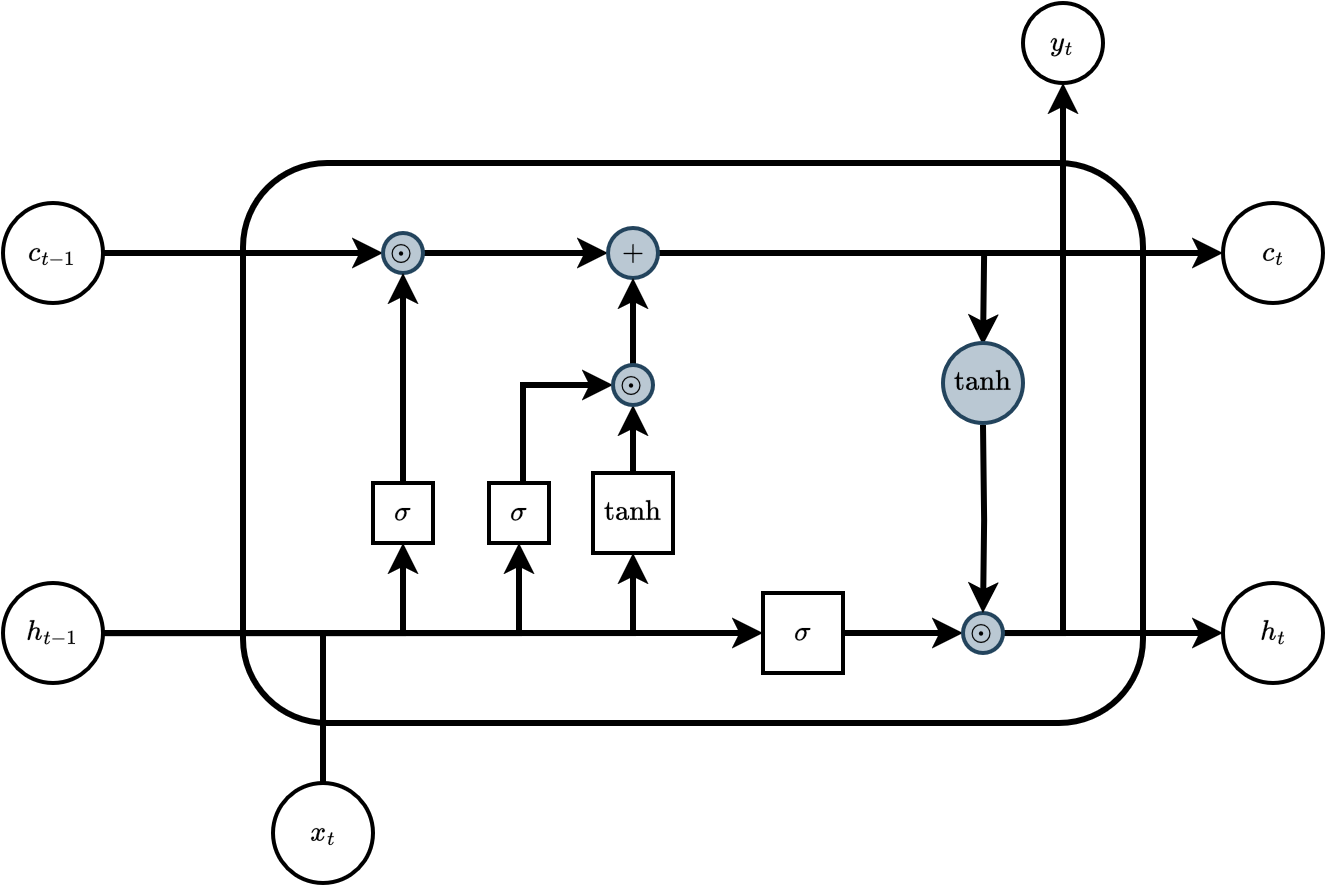
\includegraphics[scale=0.125]{assets/lstm.png}
    \caption{Information propagation through an LSTM}
    \label{fig:lstm}
\end{figure}

\begin{equation}
    \begin{aligned}
    i_t &= \sigma(W_{xi}x_t + W_{hi}h_{t-1} + W_{ci} \odot c_{t-1}+b_i) \\
    f_t &= \sigma(W_{xf}x_t + W_{hf}h_{t-1} + W_{cf} \odot c_{t-1}+b_f) \\
    c_t &= f_t \odot c_{t-1} + i_t \odot \tanh(W_{xc}x_t + W_{hc}h_{t-1}+b_c) \\
    o_t &= \sigma(W_{xo}x_t + W_{ho}h_{t-1} + W_{co} \odot c_{t}  +b_o) \\
    h_t &= o_t \odot \tanh(c_t)
    \end{aligned}
    \label{eq:lstm}
\end{equation}

Where $\odot$ refers to the elementwise product. These models can effectively model long range sequences accurately, however they are less effective with spatial information, as the inputs are in the form of a feature vector, which does not contain any spatial information. 

It is for this reason that the Convolutional LSTM~\cite{shi2015convolutionallstmnetworkmachine} architecture was developed, which combine the effective spatial learning of Convolutional Neural Networks, with the sequential modelling capabilities of LSTMs (See Equation.~\ref{eq:convlstm}). These models allow models to learn spatial transformations applied to an image over the course of a sequence, and it is for this reason that we chose this architecure for our investigation.  

\begin{equation}
    \begin{aligned}
    i_t &= \sigma(W_{xi}\ast \mathcal{X}_t + W_{hi}\ast \mathcal{H}_{t-1} + W_{ci}\odot \mathcal{C}_{t-1} + b_i) \\
    f_t &= \sigma(W_{xf}\ast \mathcal{X}_t + W_{hf}\ast \mathcal{H}_{t-1} + W_{cf}\odot \mathcal{C}_{t-1}+b_f) \\
    \mathcal{C}_t &= f_t \odot \mathcal{C}_{t-1} + i_t \circ \tanh(W_{xc} \ast \mathcal{X}_t + W_{hc} \ast \mathcal{H}_{t-1}+b_c) \\
    o_t &= \sigma(W_{xo}\ast \mathcal{X}_t + W_{ho}\ast \mathcal{H}_{t-1} + W_{co}\odot \mathcal{C}_{t}  +b_o) \\
    \mathcal{H}_t &= o_t \odot \tanh(\mathcal{C}_t)
    \end{aligned}
    \label{eq:convlstm}
\end{equation}

\section{Methods}

\subsection{Data}\label{sec:data}

In this investigation, we make use of two datasets, both deriving from the MNIST handwritten digit dataset. The first consists of 400 sequences, each containing a unique handwritten number 6, which we refer to as N6. The images were then randomly modified in an autoregressive manner, with rotation, translation, and intensity based transformations, and adding independent gaussian noise at each step, producing a sequence of 16 images, shown in Figure~\ref{subfig:n6-seq}. Images at the $4^\text{th}$ and $16^\text{th}$ positions of the sequence were then removed for use in the testing set. The second dataset, known as N3, is generated in a indentical manner but it contains the number 3, and only contains 100 sequences. This dataset is used to evaluate the performance of our model on out-of-sample data. Both sets represent their images as greyscale, 36$\times$36 pixel images. 

\begin{figure*}
    \centering
    \begin{subfigure}{0.4\textwidth}
        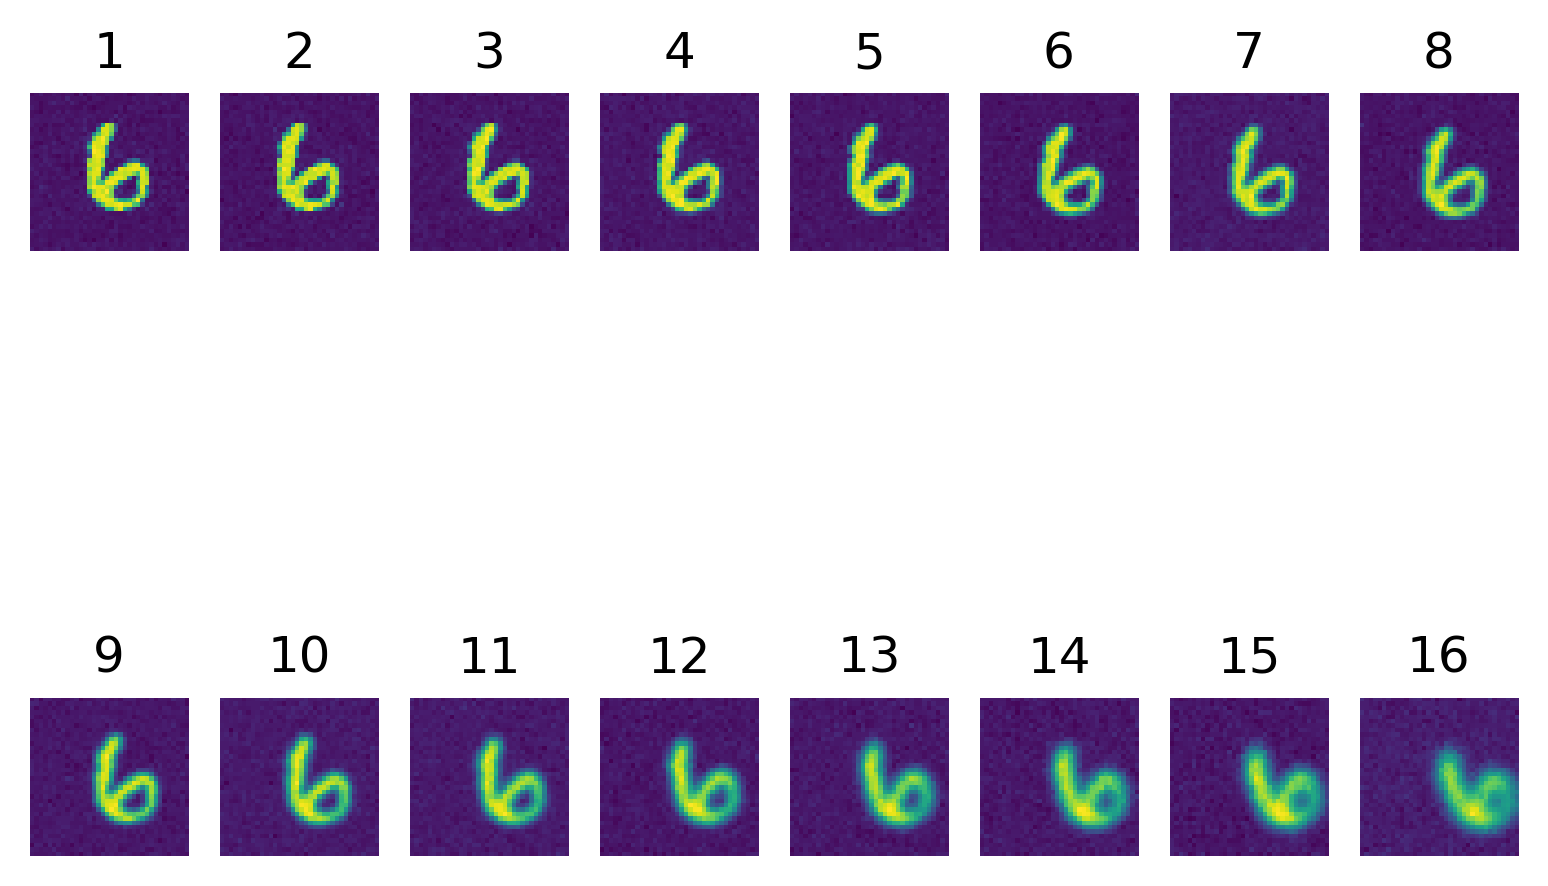
\includegraphics[width=\textwidth]{assets/seq-305.png}
        \caption{}
        \label{subfig:n6-seq}
    \end{subfigure}\hfill
    \begin{subfigure}{0.4\textwidth}
        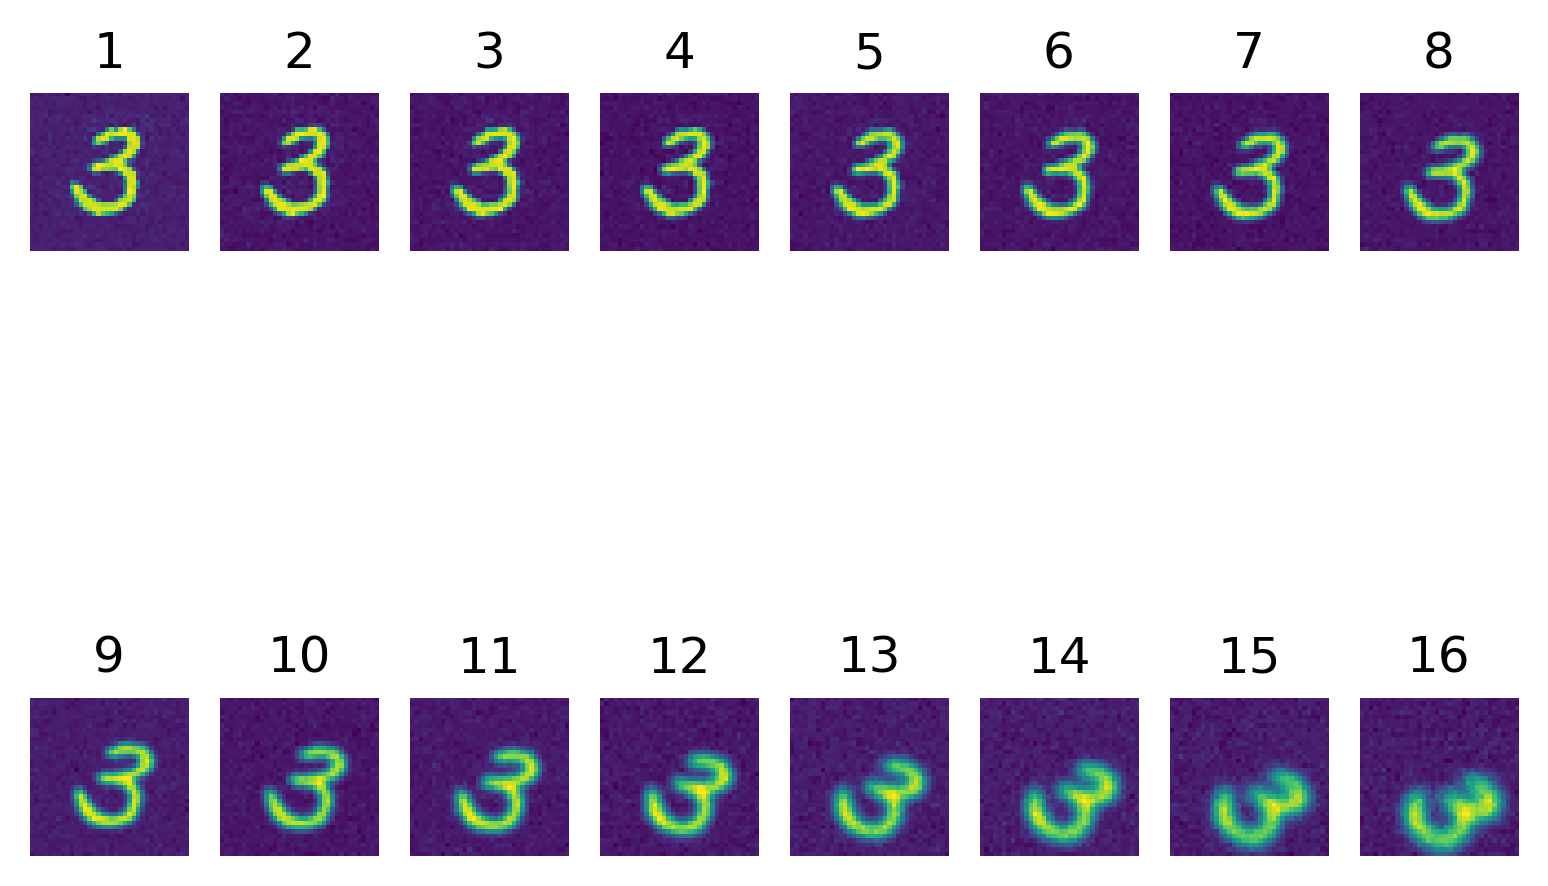
\includegraphics[width=\textwidth]{assets/n3-seq-94.png}
        \caption{}
        \label{subfig:n3-seq}
    \end{subfigure}
    \label{fig:seqs}
    \caption{Example sequences from our N6~(\ref{subfig:n3-seq}) and N3 Datasets~(\ref{subfig:n3-seq})}
\end{figure*}

\subsection{Pre-Processing}

\begin{figure}
    \centering
    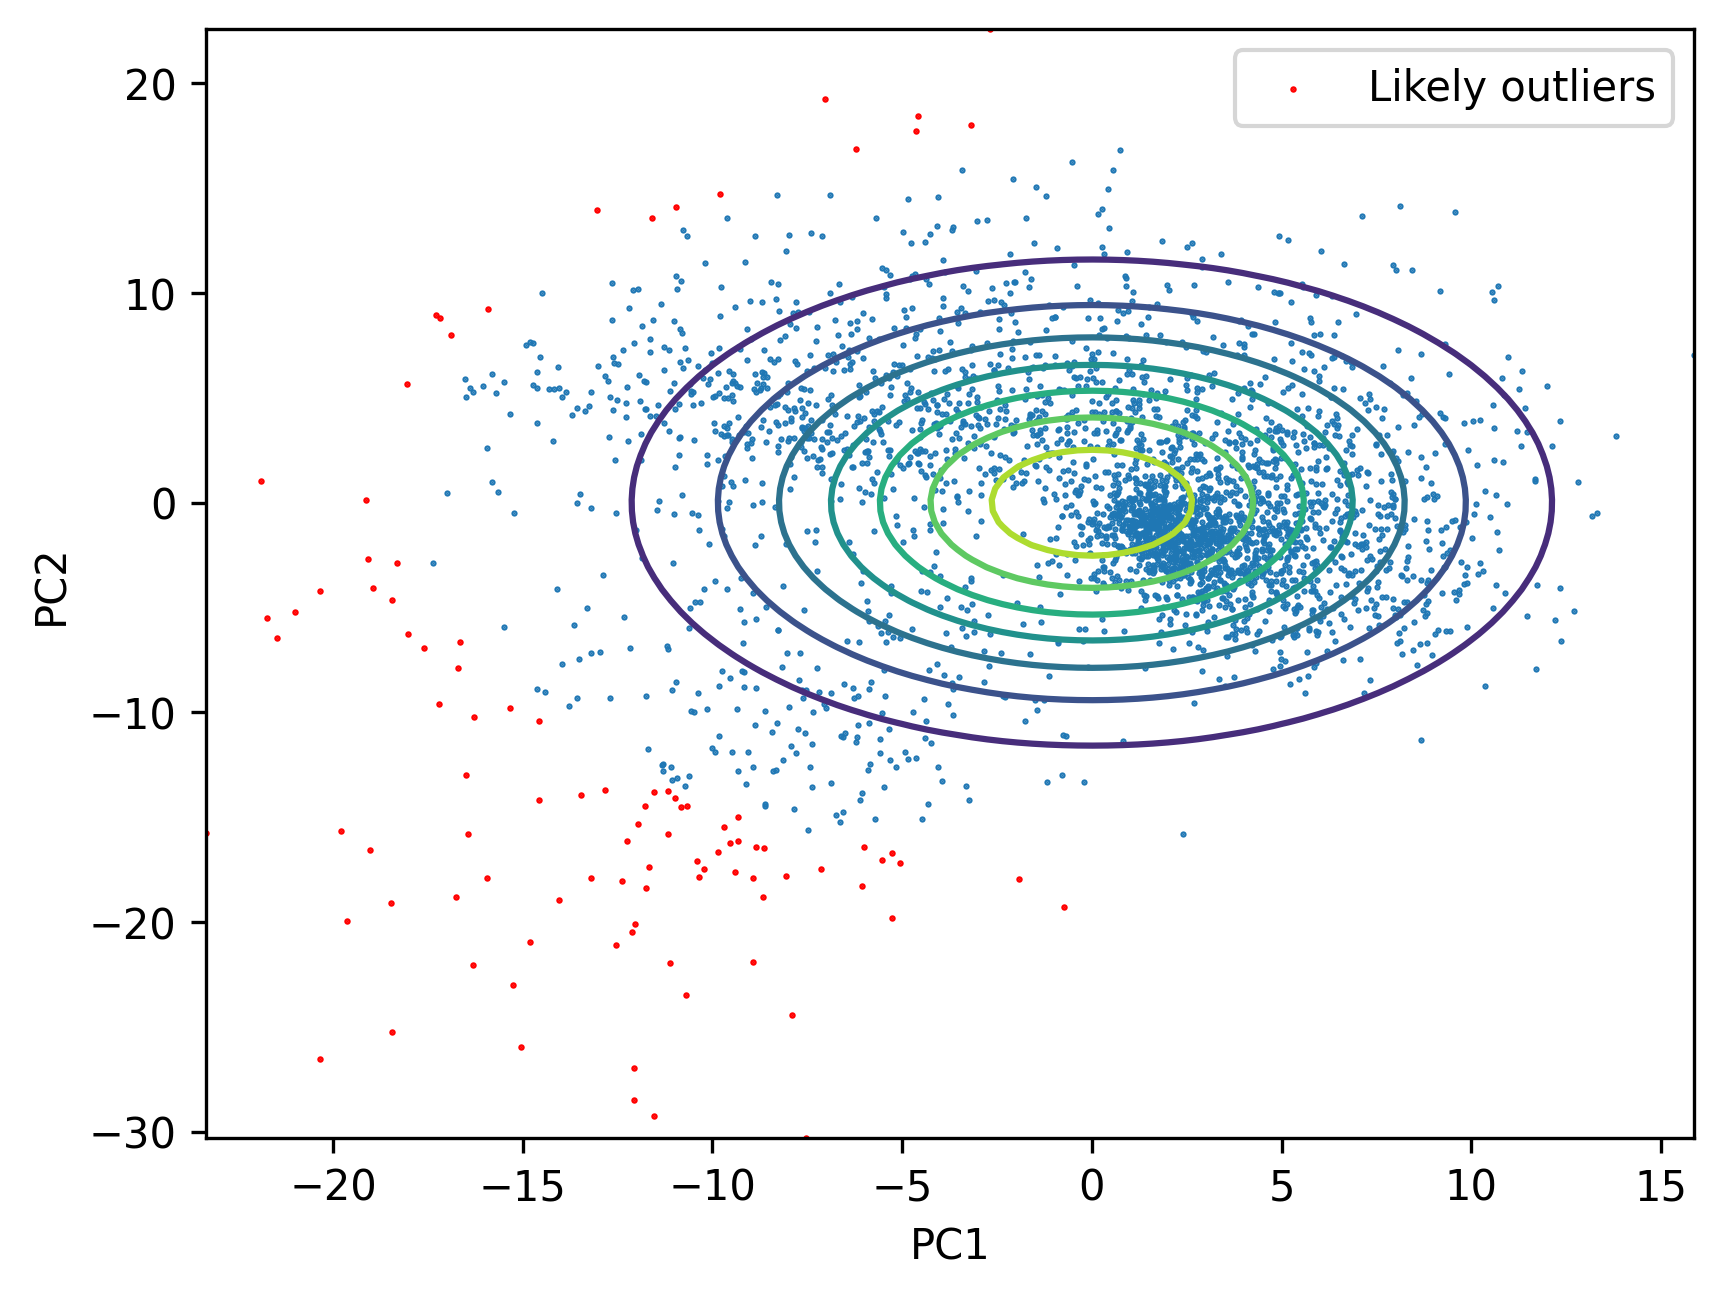
\includegraphics[scale=0.4]{assets/change-mag.png}
    \caption{PCA plot of the difference between each pair of images in a sequence across our N6 dataset.}
    \label{fig:change}
\end{figure}

We begin our pre-processing by firstly scaling the pixel intensities such that they lie in the range $[0, 1]$ for the sake of numerical stability during training. We then find any potential outliers within the N6 dataset for removal. We find potential outliers by taking the difference between consequtive images throughout the sequences found in the dataset. Then, by fitting a multivariate gaussian distribution to this information, and finding transformations which exceed three standard deviations of the mean, we find potentially anomolous transformations. We find 33 such transformations, representing approximately 1\% of our dataset, indicating they are likely anomolous as we would only expect approximately 0.3\% of transformations to exhibit such a change. Sequences containing these transformations were consequently removed.

Recall from Section~\ref{sec:data}, that at each step of the sequence, independent gaussian noise is added to the current image. In order to help the model better generalise, we denoise each of the target images in our training dataset, effectively teaching the model to ignore noise in its predictions, and focus on the spatial transformations applied to the image instead. Denoise was performed using the Non-Local Means Denoising Algorithm\cite{buades2005non} provided by the Open-CV python interface~\cite{opencv_library}. 

Finally, we also reduce the length of our sequences from 16 to 3, as this will enable the model to learn the future transformation given only the previous two. This also has the added effect of drastically reducing the time spent training our models. Subsequences which predict the $4^\text{th}$ and $16^\text{th}$ images comprise our test set, and sequences containing the test images as part of their inputs are removed alltogether. 

From these pre-processing steps, we arrive at 4 different training datasets. The first of which includes outliers and noise in the target images, refered to as the fully processed dataset, a dataset featuring the removal of outliers found earlier, known as the cleaned dataset, the dataset with denoised target images, and the base dataset with no pre-processing other than the reducition in sequence length. 

\subsection{Training}

We test our convolutional LSTM model with both the Rectified Linear Unit (ReLU), and hyperbolic tangent ($\tanh$) output activation functions, with 1 to 7 layers, and 1 to 100 kernels. We also vary the learning rate randomly from $1\mathrm{e}-5$ and $0.1$, and batch size from 32 to 256. Each trial of our experiment also randomly selects one of the 4 datasets we outlined in the previous section, in addition to the optimisation algorithm used during training. Between each layer of our model, we also include batch normalisation to assist with regularisation. 

We evaluate the performance of our models using the Mean-Squared-Error metric, as it captures pixel level differences between images, and we test on both the selected n6 test dataset, and the full, unprocessed n3 dataset at each training episode. 

The training itself took place over 20 episodes on a single nvidia RTX A6000 GPU, with 264 GB of RAM, and performing 200 trials in total. 

We also test our best model on an augmented test dataset consisting of different types of noise at different intensities. We chose to test Gaussian, Poisson, and ``salt and pepper'' noise (See Figure~\ref{fig:noise}), at 100 levels of intensity, and capture the average test loss on both the n6, and n3 test datasets. These types of noise are accurate models of the forms of noise we see in real world images, and we hope this experiment will characterise the robustness of our models to noise. Furthermore, we also remove a randomly selected region of each image in a separate test to further investigate its robustness. At each step of this experiment, we increase the size of the missing region by a single pixel, until the entire image is removed. This transformation is only applied to the input images. 

\begin{figure}
    \centering
    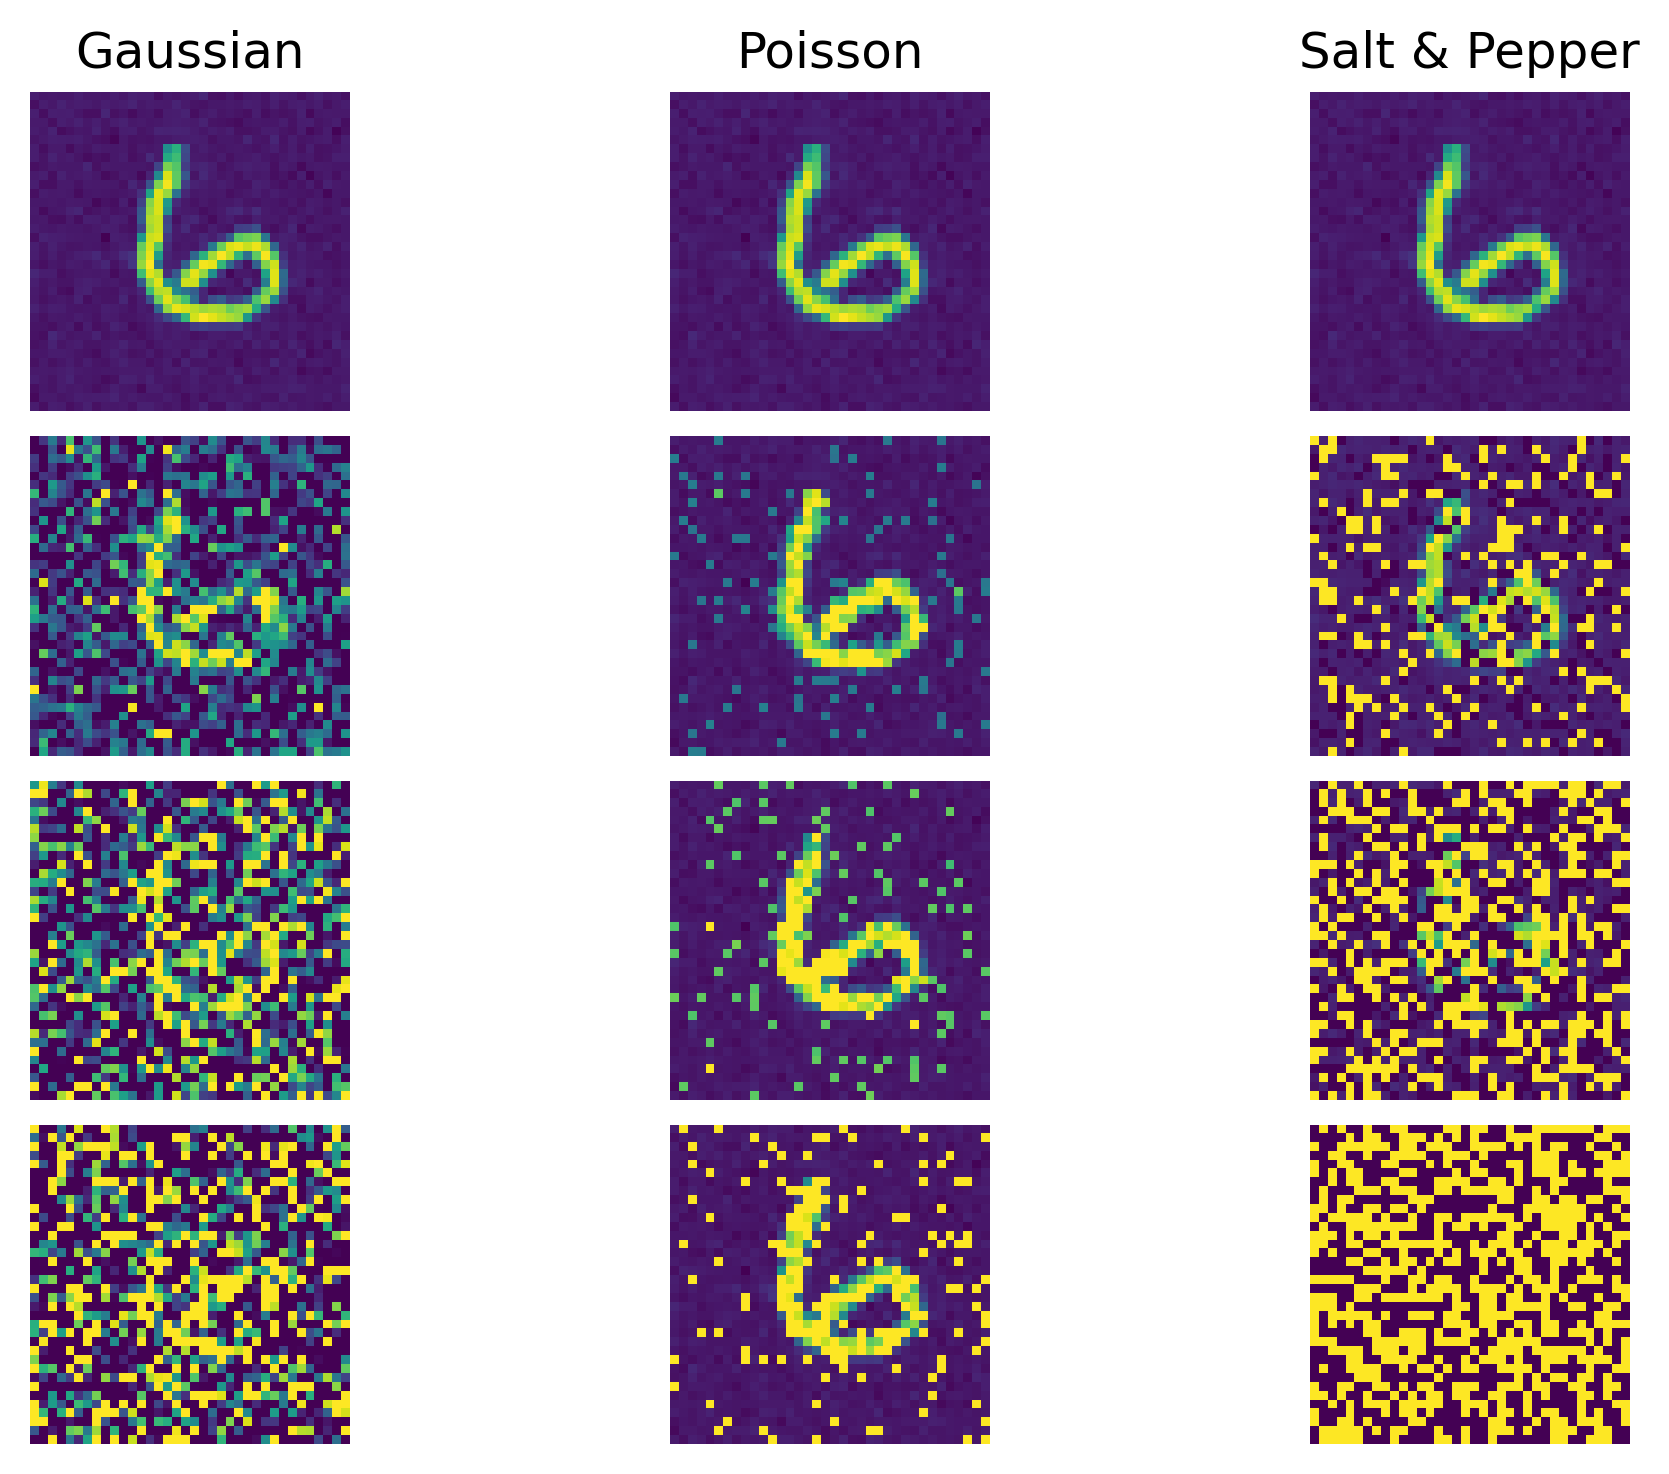
\includegraphics[width=0.3\textwidth]{assets/noise.png}
    \caption{Each of the types of noise applied to a sample image, at different intensities, the top row has no added noise (intensity = 0), and the bottom row has full intensity (intensity = 1) }
    \label{fig:noise}
\end{figure}

\section{Results}

\begin{figure}
    \centering
    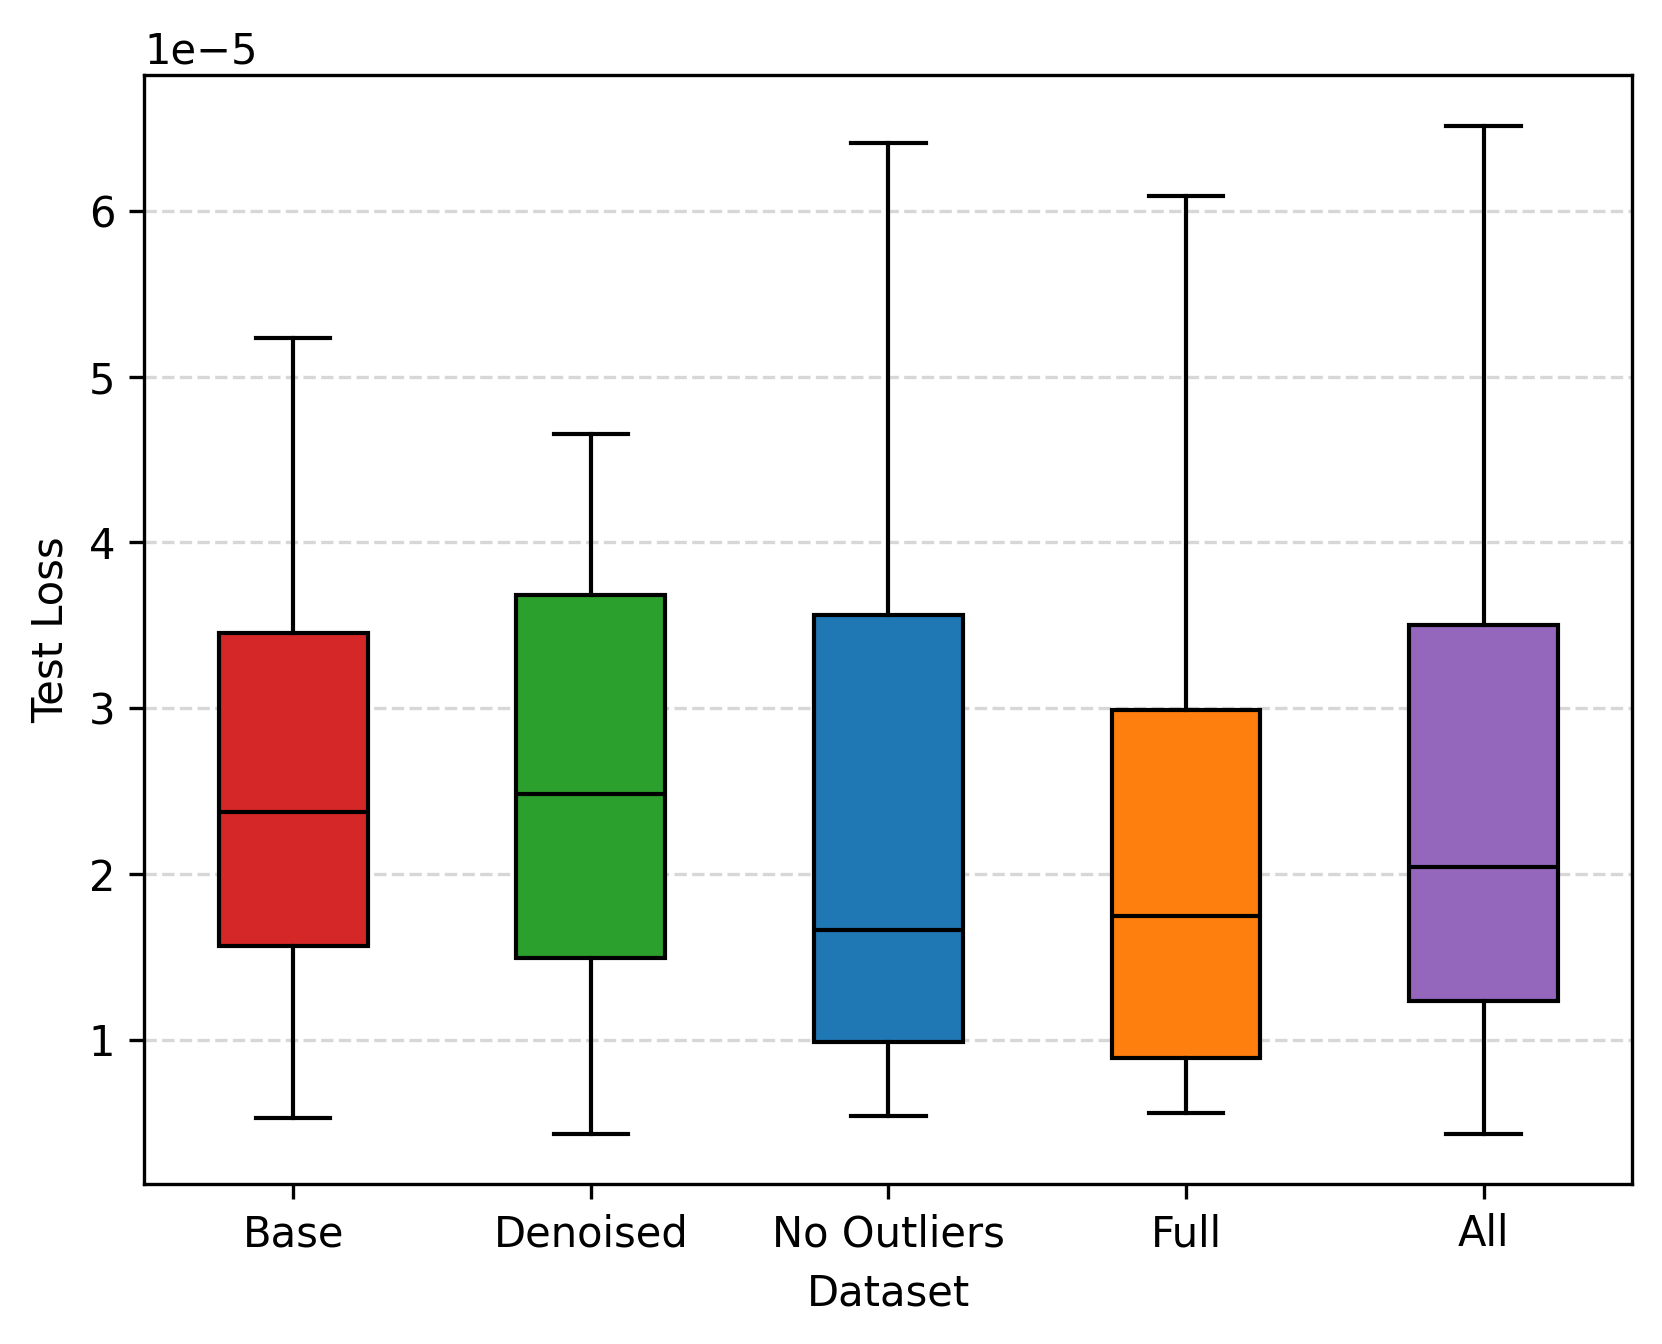
\includegraphics[scale=0.4]{assets/results-bar.png}
    \caption{Distribution of test losses achieved by our model on the different datasets}
    \label{fig:loss}
\end{figure}

Throughout our experiment of 200 training runs, we found 30 runs overfitted the training dataset, and only predict empty images during testing. These runs were consequently removed, leaving us with 170 runs in total. Of these 170 runs, 40 were performed on the base dataset, 44 on the denoised dataset, 50 on the dataset with outliers removed, and 36 on the fully processed dataset. The average test loss on both the N3 and N6 datasets are shown in Figure~\ref{fig:loss}, note that outliers have been removed from the graph for the sake of readability. 

Of each of these datasets, we found the dataset with outliers removed achieved the lowest median test loss over all runs however it also exhibits the greatest spread in this metric. The fully processed dataset however, had the lowest variance in test loss, while also having a high maximum. Interestingly, the best test loss seen across all trials of our experiment, was performed on the denoised dataset. However, on average, it doesn't seem to yield much of an improvement over our base dataset. This suggests that its performance may be an effect of the hyperparameters used, or the random weight initialisation. 

When looking at the images produced by this model (Figure~\ref{fig:quali}), we see that it captures the spatial transformations well across both datasets, however it sometimes struggles with the intensty of pixels. Furthermore, we also see that it struggles with predicting noise, especially when predicting images towards the end of a sequence, which is largely to be expected, as it was trained on the denoised dataset. 

\begin{figure*}
    \centering
    \begin{subfigure}{0.4\textwidth}
        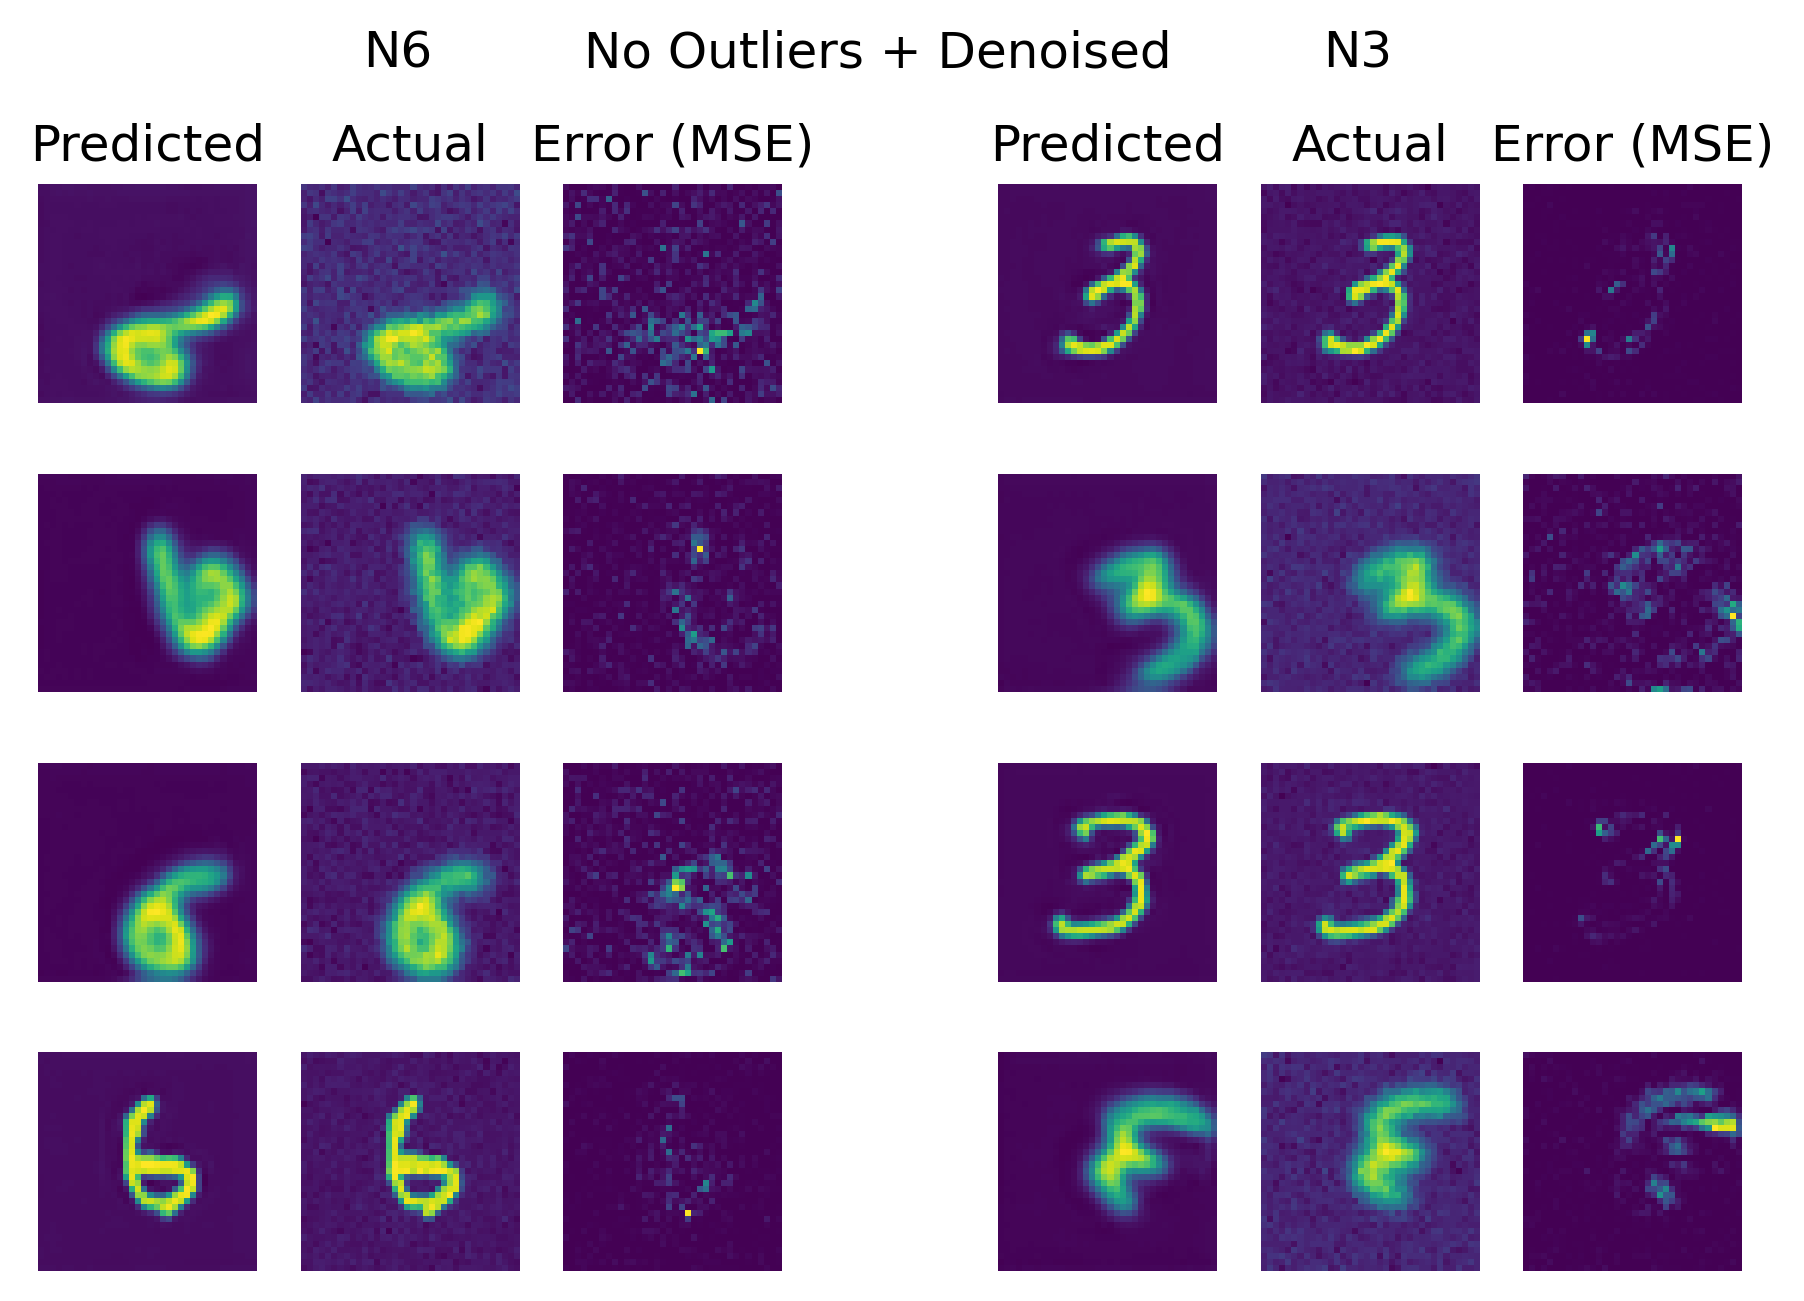
\includegraphics[width=\textwidth]{assets/best-gen.png}
        \caption{Predicted images from both test sets, and the mean squared error between the output, and its target} 
        \label{fig:error}
    \end{subfigure}\hfill
    \begin{subfigure}{0.4\textwidth}
        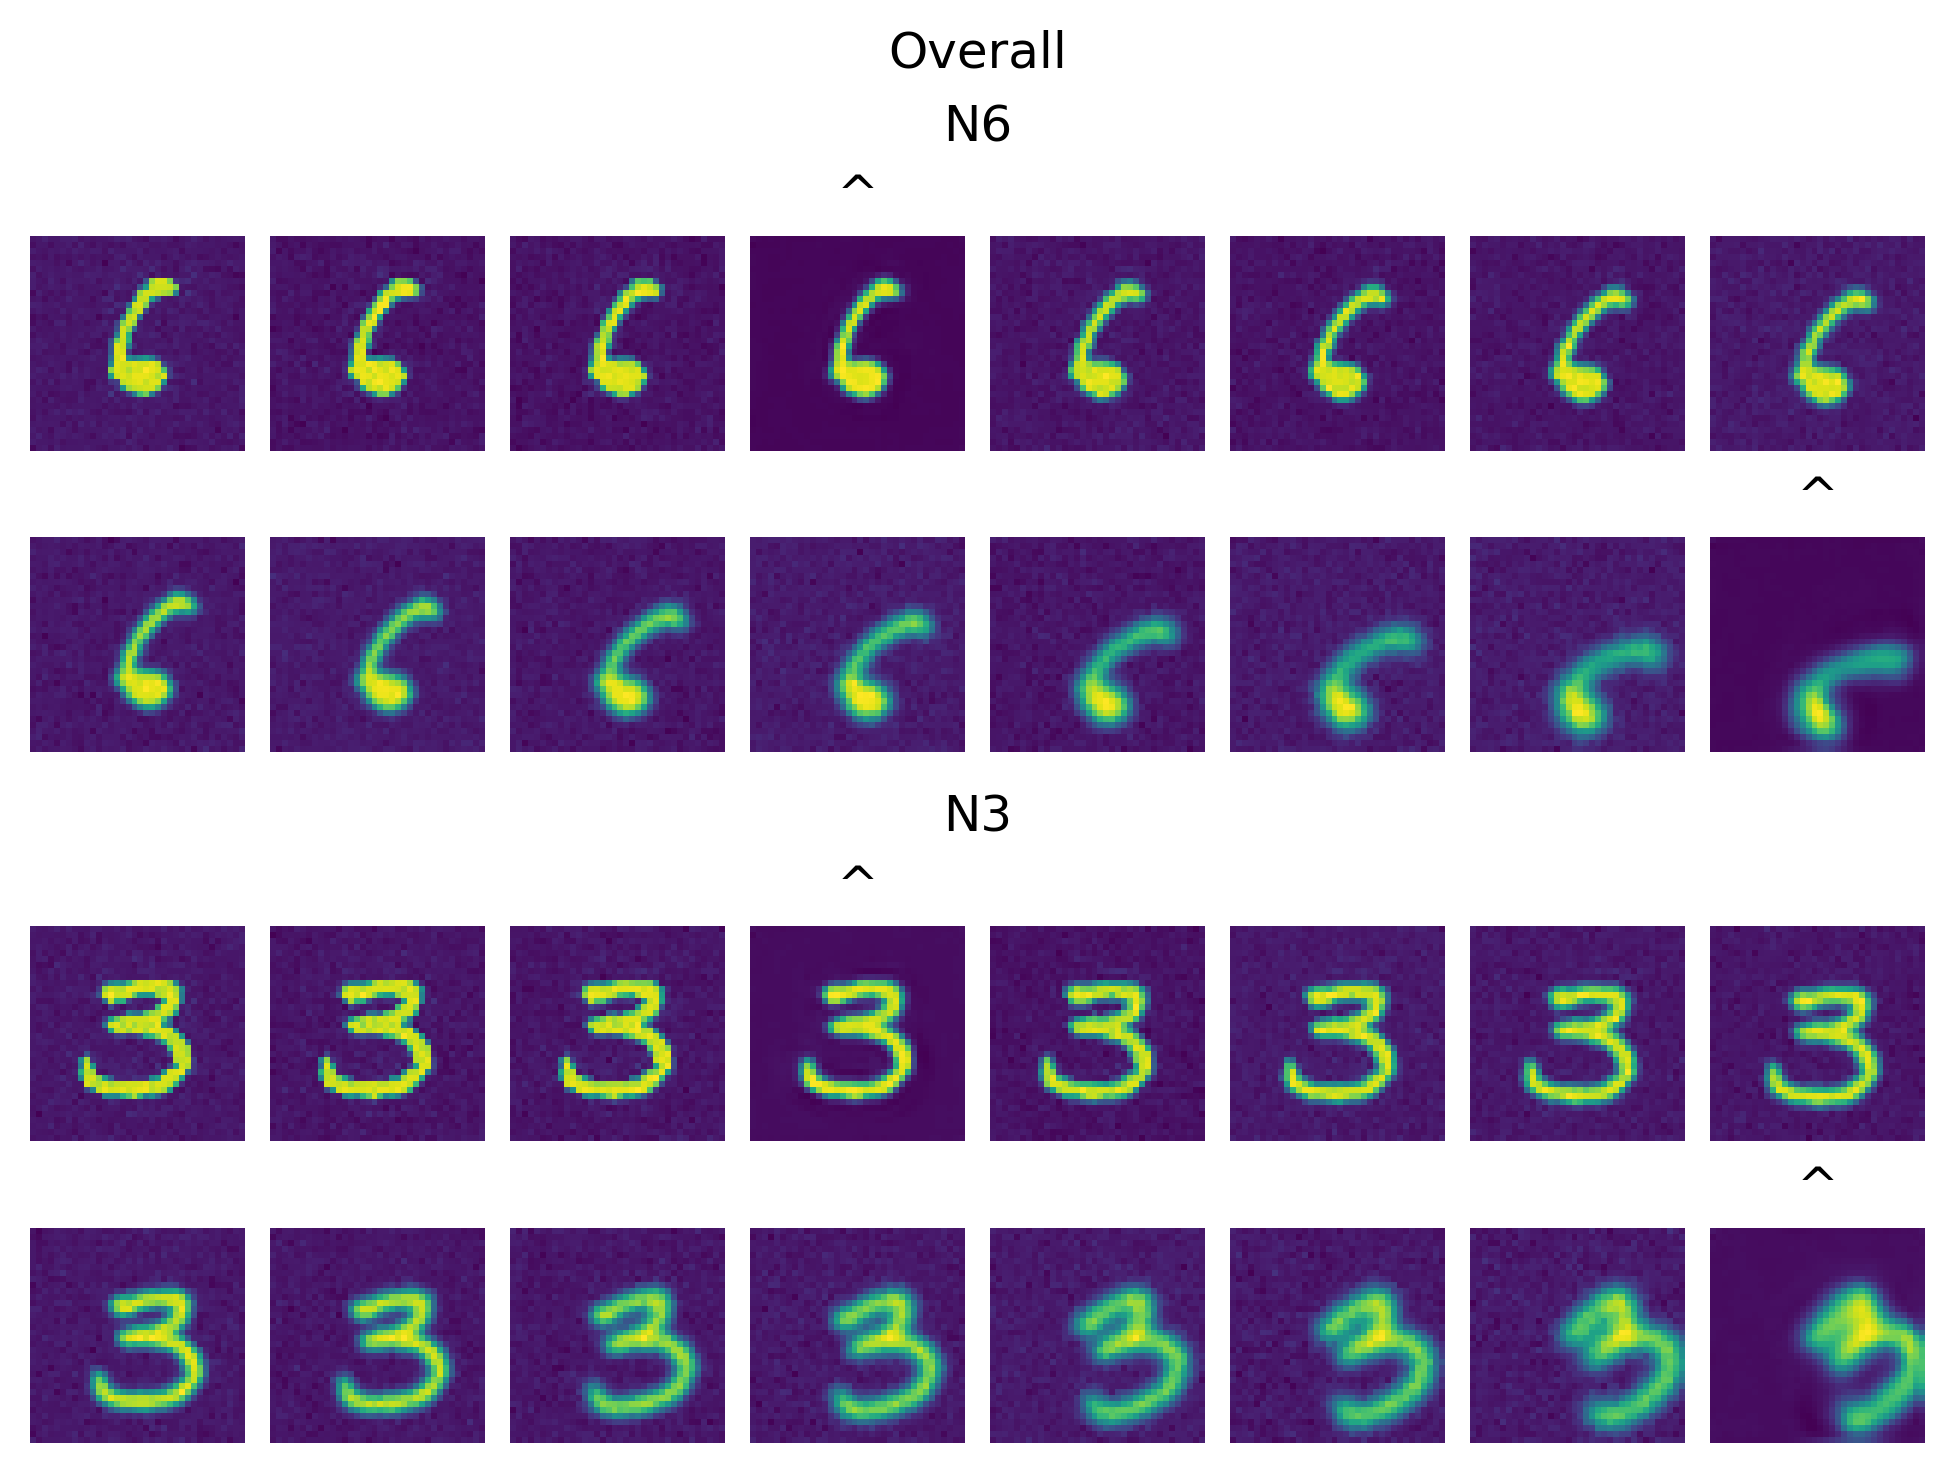
\includegraphics[width=\textwidth]{assets/best-in-context.png}
        \caption{Predicted images in context, where a carat ($~\hat{}~$) above an image denotes it as being the output from our model} 
        \label{fig:in-context}
    \end{subfigure}
    \caption{Images generated by our best performing model, including mean squared error between predictions, and ground truth~(\ref{fig:error}), and the predicted images in context~(\ref{fig:in-context}) }
    \label{fig:quali}
\end{figure*}

Our best model used 4 LSTM layers, with 71 kernels, and the ReLU activation function as shown in Table~\ref{tab:results}. We find that of all the best runs throughout our experiment also took similar values for the number of layers. However, there is significant variance in the optimal number of kernels. For example, on our base dataset, we achieved the best test loss with 10 kernels in total however the best overall result we obtained, used 71 kernels. Models trained on both the cleaned, and the fully processed datasets achieved their best results with approximately 40 kernels. This suggests that when working with unprocessed data, a less complex model is preferable at the cost of worse performance. However, when working with processed data, our models require additional complexity, and enable it to better model the transformations applied to the images throughout the sequence. 


\begin{table*}[]
    \begin{tabular}{@{}cllllllll@{}}
        \toprule
        \multirow{2}{*}{\textbf{\begin{tabular}[c]{@{}c@{}}Training\\ Dataset\end{tabular}}} & \multicolumn{6}{c}{Parameters} & \multicolumn{2}{c}{Test Loss} \\ \cmidrule(l){2-9} 
         & \multicolumn{1}{c}{\textbf{Batch Size}} & \multicolumn{1}{c}{\textbf{Activation}} & \multicolumn{1}{c}{\textbf{Layers}} & \multicolumn{1}{c}{\textbf{Kernels}} & \multicolumn{1}{c}{\textbf{LR}} & \multicolumn{1}{c}{\textbf{Optimizer}} & \multicolumn{1}{c}{\textbf{N6}} & \multicolumn{1}{c}{\textbf{N3}} \\ \midrule
        Base & 224 & tanh & 5 & 10 & 0.03719 & RAdam & 4.69e-6 & 5.25e-6 \\
        Denoised & 254 & ReLU & 4 & 71 & 0.004778 & Adamax & 3.69e-6 & 4.32e-6 \\
        Removed Outliers & 214 & ReLU & 4 & 42 & 0.0010676 & Adamax & 4.52e-6 & 5.41e-6 \\
        Fully Processed & 216 & ReLU & 4 & 41 & 0.004656 & Adam & 3.86e-6 & 5.57e-6 \\ \bottomrule
        \end{tabular}
    \caption{The hyperparameters and the average mean-squared-error achieved by the best performing model trained on each dataset.}
    \label{tab:results}
\end{table*}

Our investigation into our models robustness, the results of which are shown in Figure~\ref{fig:robust-results} suggest our model is robust to both poisson, and gaussian noise with an intensities of less than approximately 0.2. However, once the intensity exceeds this, it begins to drastically rise. The salt and pepper noise however, has a more significantly impact on its performance. This form is noise is generated by setting random pixels from the image, and randomly setting them to either black or white. The intensity parameter controls the probability of any given pixel in the image being set to noise. As we increase intensity, fewer pixels from the image remain, meaning that there is less information for the model to work with. Throughout each of the types of noise, the models performance on the N3 dataset is worse than the N6 dataset. This disparity also increases as we increase the intensity of noise, and is most apparent in the poisson noise test. The effects of missing regions within the image are shown in Figure~\ref{fig:missing-results}, and we again see a disparity between the N6, and N3 datasets. Interestingly, we also see that as more approximately half of the image is removed, the loss decreases below the loss achieved on the unaugmented dataset. This may be due to the model predicting a blank image when the size of the removed region exceeds 


\begin{figure*}
    \centering
    \begin{subfigure}{0.4\textwidth}
        \centering
        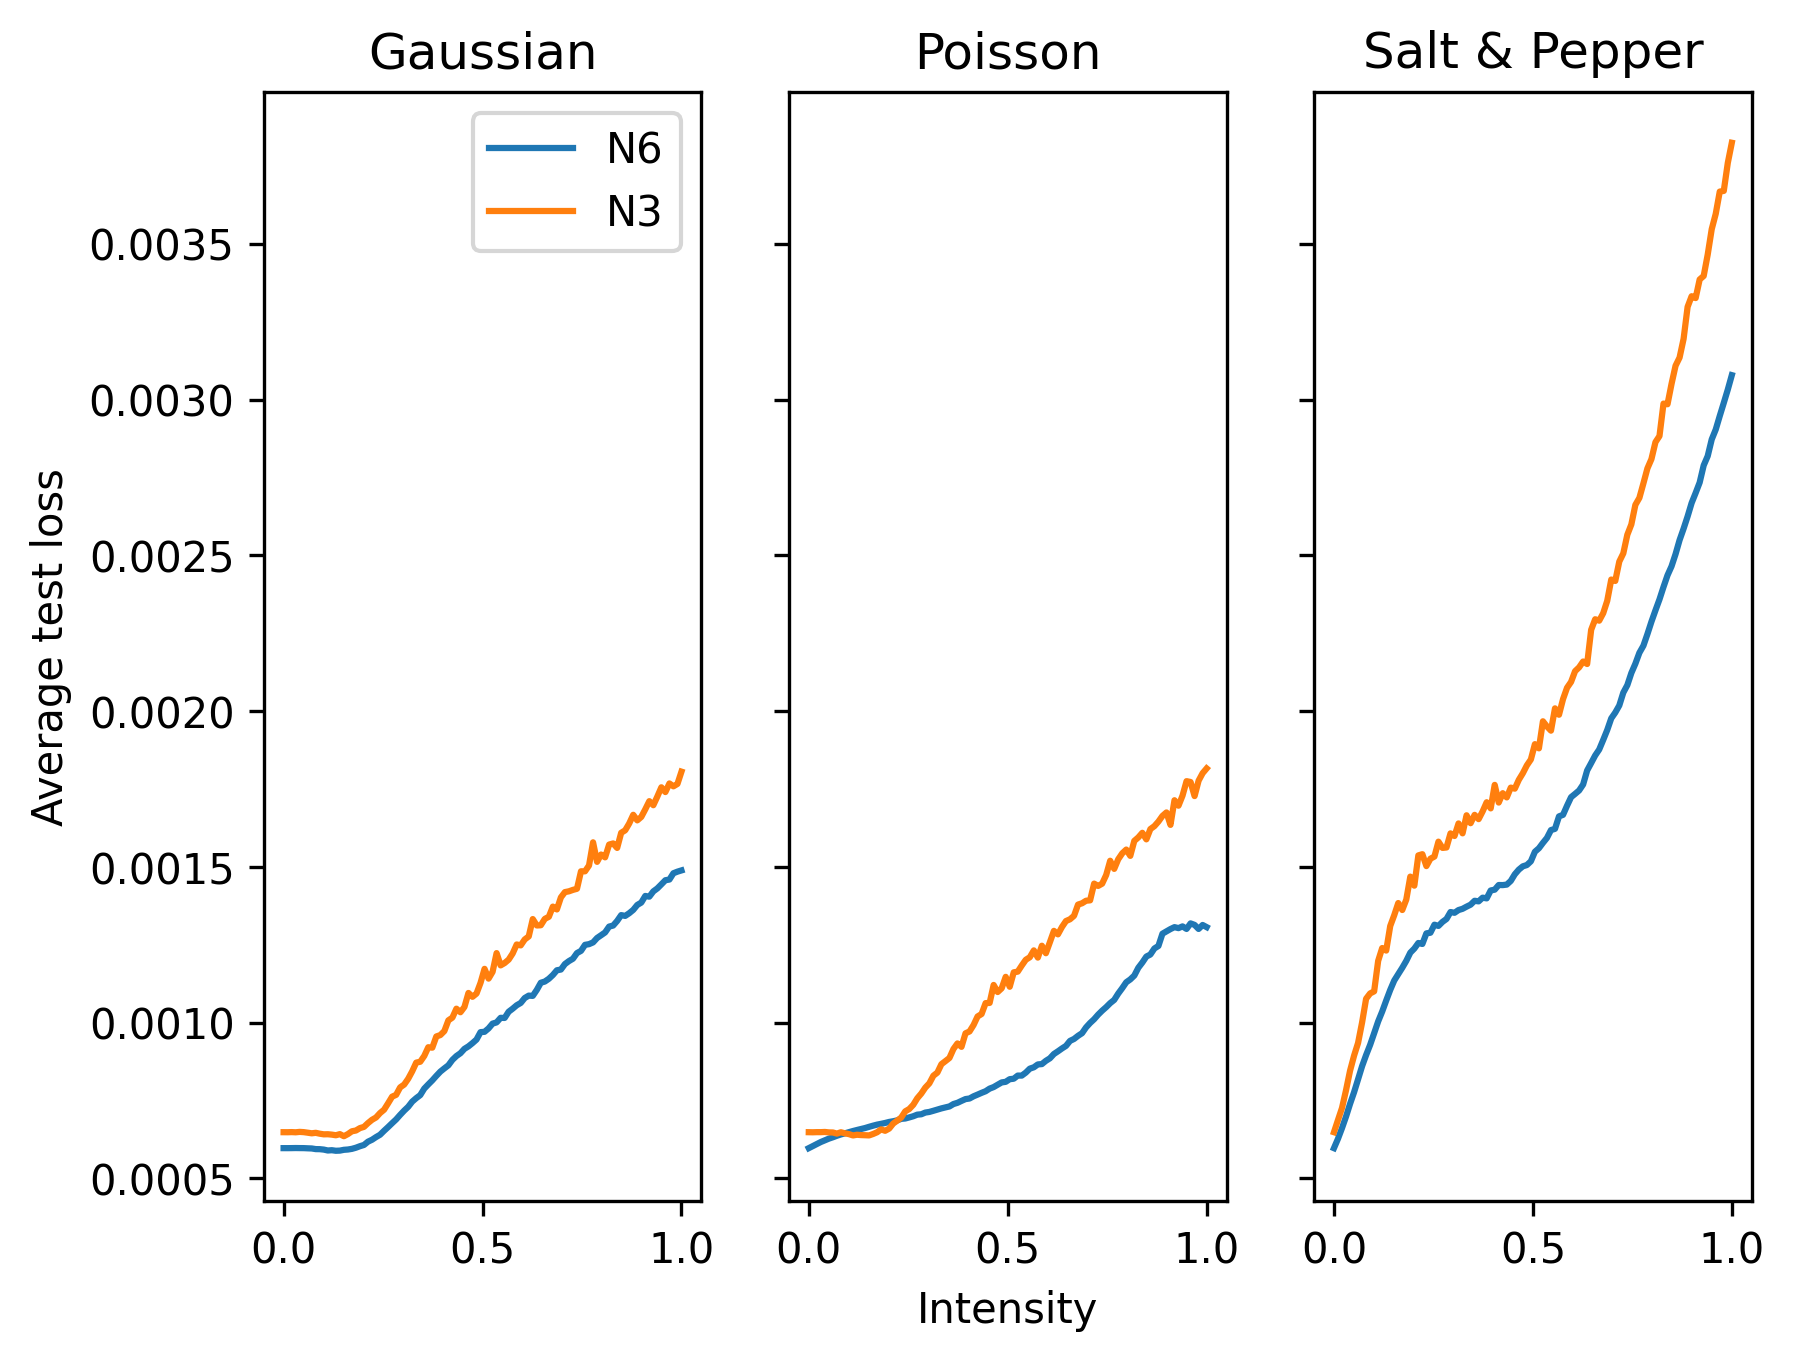
\includegraphics[width=0.9\textwidth]{assets/noise-results.png}
        \caption{The average test loss with regards to the intensity and kind of noise applied}
        \label{fig:robust-results}
    \end{subfigure}\hfill
    \begin{subfigure}{0.4\textwidth}
        \centering
        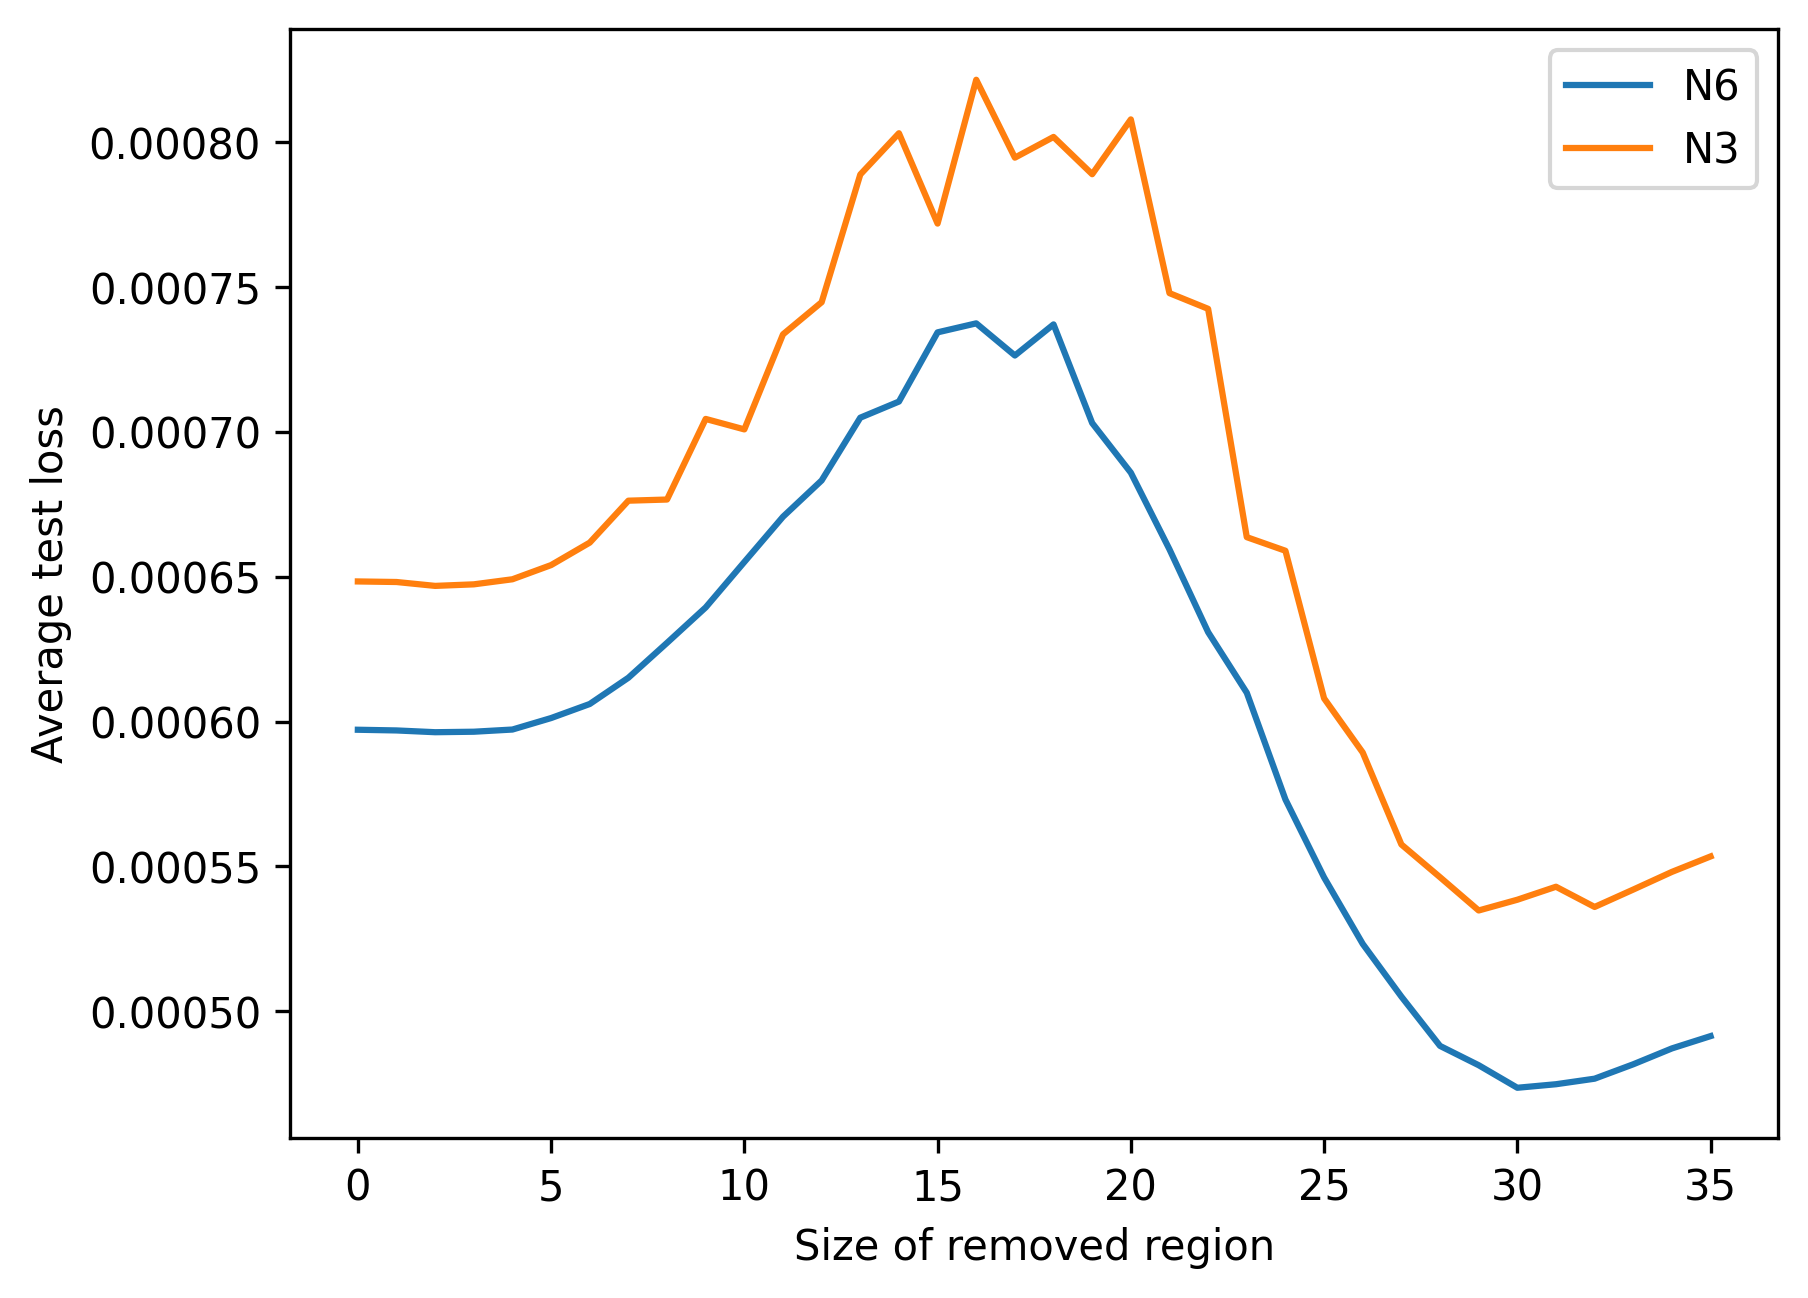
\includegraphics[width=0.9\textwidth]{assets/missing-data.png}
        \caption{Average test loss with randomly removed regions of the image}
        \label{fig:missing-results}
    \end{subfigure}
    \caption{Graphs quantifying the robustness of our best performing model to both noise (\ref{fig:robust-results}) and missing data (\ref{fig:missing-results}).}
    \label{fig:robustness}
\end{figure*}

\section{Conclusion}

In this report, we have outlined our implementation of a Convolutional Long-Short-Term-Memory model for use in a image sequence modelling task, and the results we obtain from our experiments. We perform both quantitative, and qualitative analysis of the data we obtain, and evaluate how resiliant our model is to images with various types of noise at different intensities and varying amounts missing data in the test images. 

Future work in this field could investigate how other models for spatial-temporal learning perform in comparison to our model, such as the models developed as part of the OpenSTL benchmark\cite{tan2023openstl,gao2022simvp,tan2022simvpv2,tan2023temporal}, in addition to Recurrent Inference Machines~\cite{putzky2017recurrentinferencemachinessolving}. In addition to this, the effect of other metrics, such as Peak Signal-to-Noise ratio, structural similarity index measure, and perceptual loss, as we only used mean squared error to evaluate our models performance. Furthermore, as LSTMs are designed for use in long term sequence modelling tasks, and we work with smaller sequences, other models such as RNNs could be investigated to see if the computational complexity of the model could be reduced.

\printbibliography

\end{document}